\documentclass[12pt, a4paper]{article}
\title{A Technical Note on Atomic Beam Fluorescence Measurements for the Design of a Single Atom Microscope}
\usepackage{graphicx}
\usepackage{url}
\usepackage{wrapfig}
\usepackage{mathrsfs}
\usepackage{amssymb}
\usepackage{array}
\usepackage[font={small}]{caption}
\usepackage{geometry}
\geometry{margin=1in}
\author{Kristen Parzuchowski}
\begin{document}
\maketitle
\begin{abstract}
The Single Atom Microscope (SAM) will be used to measure rare nuclear reaction rates relevant for nuclear astrophysics. SAM will capture and detect all of the product atoms of the reactions of interest inside of a solid film of Neon. A detailed understanding of the number of atoms embedded in Neon is necessary in order to determine the intrinsic brightness of the product atoms in medium. This technical note describes the current status of the atom number in medium calibration including all assumptions made.
\end{abstract}
\section{Introduction}
The Single Atom Microscope is a new detector we are designing in order to measure rare nuclear reactions relevant for Nuclear Astrophysics. This detector captures and detects all product atoms of the reaction of interest inside of solid Neon. Our detection is highly efficient, because the solid Neon will capture all product atoms, highly selective, because the product atoms are selected using resonant laser excitation, and highly sensitive, because there is a large shift between the emission and excitation spectrum of the product atom which significantly suppresses scattered light background from the laser. My primary interest is in determining exactly how sensitive our technique is, or what the intrinsic brightness of our product atoms in solid Neon is. A low intrinsic brightness will require long integration times in order to detect single atoms. 

A number of things must be known in order to determine the intrinsic brightness of the product atoms in medium including:
\begin{itemize}
\item \textbf{Number density of atoms embedded in medium}
\item Illumination laser intensity and beam profile
\item Light collection efficiency
\item Background sources present
\end{itemize}
This technical note focuses on calibrating the number density of atoms embedded in medium. To do this I perform atomic beam fluorescence(ABF) measurements and simulations. 
\section{Atomic Structure of Yb}
Ytterbium(Yb) is a metallic chemical element in the lanthanide series. The valence shell of Yb contains two electrons ([Xe]4f$^{14}$6s$^{2}$).
\subsection{Isotopic Abundance}
The Yb in our studies is in natural isotopic abundance, given in the table below.
\begin{center}
\begin{tabular}{||c|c|c||}
\hline
Isotope & Abundance & Nuclear Spin, I\\
\hline \hline
168 & 0.126 \% & 0\\
\hline
170 & 3.023\% & 0 \\
\hline
171 & 14.216\% & 1/2 \\
\hline
172 & 21.754\% & 0 \\
\hline
173 & 16.098\% & 5/2 \\
\hline
174 & 31.896\% & 0 \\
\hline
168 & 12.887\% & 0 \\
\hline
\end{tabular}
\end{center}
\subsection{Hyperfine Structure}
The hyperfine structure of an atom is a result of the interaction of the nucleon spin with the electron spin. For a given total electron angular momentum, $J$, and a total nuclear spin angular momentum, $I$, a total angular momentum can be calculated:
\begin{equation}
\vec{F} = \vec{J} +\vec{I}
\end{equation}
For Yb, $J=1$. Only isotopes with nonzero nuclear spin will be split into a hyperfine structure of states. For $^{171}$Yb, $F=1/2,3/2$ and for $^{173}$Yb, $F=3/2,5/2,7/2$.
\subsection{Frequency Splittings}
The frequency splittings of Yb have been studied and measured a number of times before, so these values can be found in published papers. In the table below, the values I gathered from [3] are listed.
\begin{center}
\begin{tabular}{||c|c||}
\hline
Isotope & Shift from $^{174}$Yb (MHz)\\
\hline\hline
176 & -509.310(50) \\
\hline
173 (F=5/2) & -253.418(50) \\
\hline
173 (F=3/2) & 515.975(200) \\
\hline
172 & 533.309(53) \\
\hline
173 (F=7/2) & 587.986(56) \\
\hline
171 (F=3/2) & 832.436(50) \\
\hline
171 (F=1/2) & 1153.696(61) \\
\hline
170 & 1192.393(66) \\
\hline
168 & 1887.400(50) \\
\hline
\end{tabular}
\end{center}

\section{Apparatus}
The apparatus used for these studies is the setup for the Single Atom Microscope. 
\subsection{Atomic Oven}
\begin{wrapfigure}{r}{0.45\textwidth}
\vspace*{-5mm}
  \includegraphics[scale=0.37]{vaporpressure_ybmg.png}
  \vspace*{-5mm}
  \caption{Vapor Pressure (Pa) of Yb (Blue) and Mg (Green) as a function of Temperature ($^{\circ}$C). Data is extracted from equations given in [1].}
\end{wrapfigure}
The atomic oven is the source of Yb for our atomic beam. This oven is rated for 450$^{\circ}$C, which at this operating temperature will well satisfy our requirements for Yb number density in vacuum. From theory [2] of effusive beam sources,  atomic beam flux has the relation: $Flux \propto \frac{P}{\sqrt{m}}$, where $P$ is the vapor pressure of the atoms and $m$ is the mass of atom. The vapor pressure of Yb and Mg at various temperatures is shown in figure 1. As Mg has a smaller mass and a larger vapor pressure than Yb, we can expect that this atomic oven will also satisfy the number density requirements for Mg. 

The oven design is shown in figure 2. The atomic beam effuses through a long cylindrical tube aperture on the oven. If $l$, the length of the cylindrical tube, is much larger than, $r$, the radius of the aperture, the number of atoms emerging from the source per unit time can be predicted theoretically by [2]:
\begin{equation}
Q = \frac{2}{3}\frac{r}{l}n\bar{v}A,
\end{equation}
where $n$ is the number of atoms per unit volume, $\bar{v}$ is the mean atomic velocity and $A$ is the area of the source slit. In our case, $l = 0.500"$ and $r = 0.0625"$, so our assumption is satisfied fairly well.
\begin{figure}[h]
\centering
\captionsetup{justification=centering}
  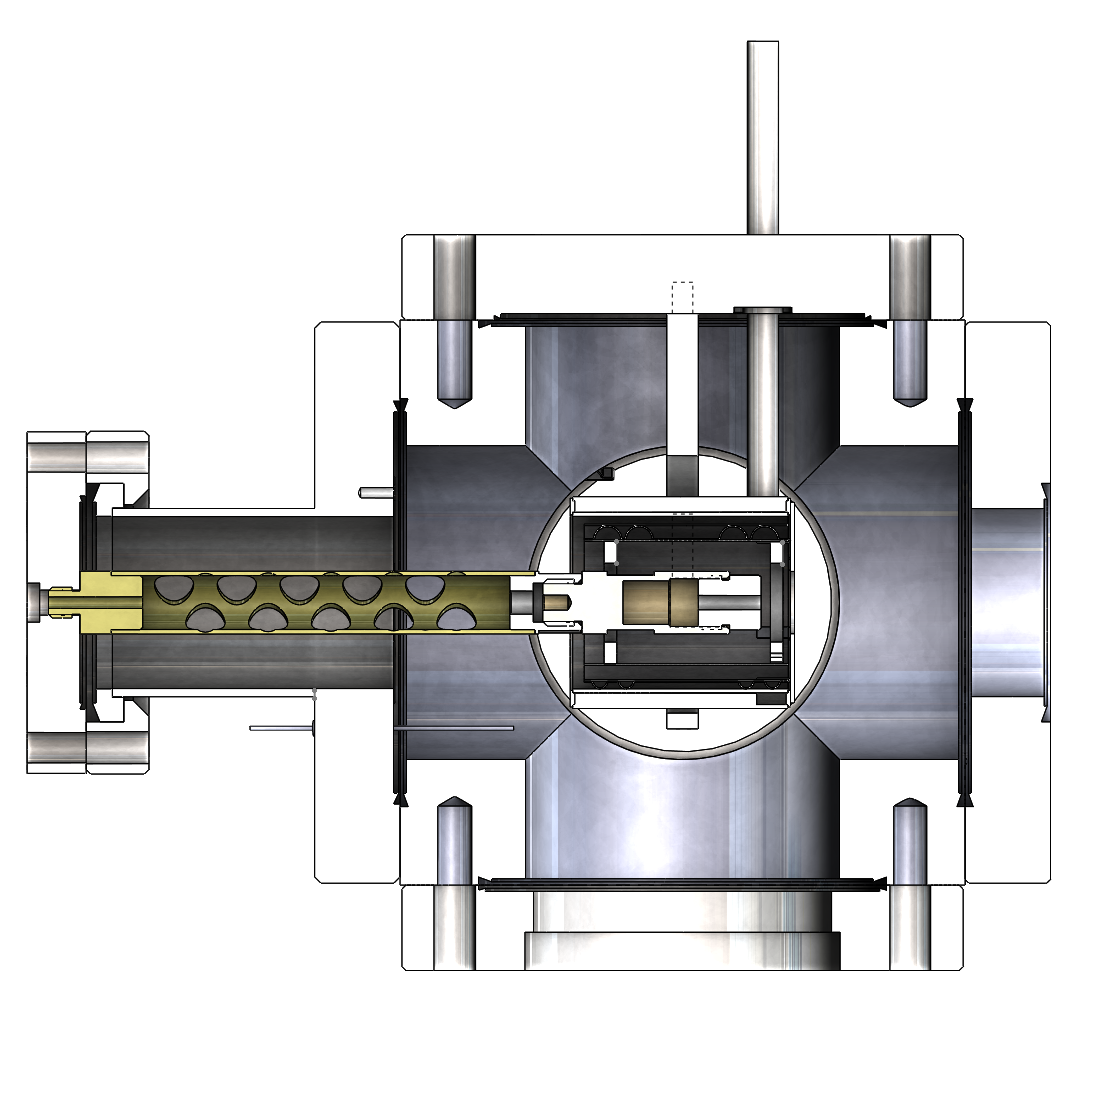
\includegraphics[scale=0.22]{ybOvenCrosssection.PNG}
  \vspace*{-3mm}
  \caption{Yb oven cross section}
\end{figure}

\subsection{Atomic Beam}
The atomic beam exits the oven aperture and traverses through the SAM vacuum system. This vacuum systems consists of a straight path from the oven aperture to the cryostat. The diameter of the vacuum chamber is $\sim 2.3"$, allowing for a maximum atomic beam diameter of that size. Any atoms that hit the surface of the vacuum chamber will stick to the surface. I approximate the angle of divergence for the atomic beam through the assumption that $\theta_{max} = \tan^{-1}\frac{2r}{l}$. According to theory [2], the intensity of the atomic beam resembles a cosine distribution. I approximate the spatial distribution of the atomic beam as a uniform distribution.

The cross section for an atom is given by:
\begin{equation}
\sigma(\nu) = \pi r_e c f \mathscr{L}(\nu)
\end{equation}
where $r_e$ is the classical electron radius, $c$ is the speed of light, $f$ is the oscillator strength and $\mathscr{L}(\nu)$ is the lineshape of the transition. An atom's natural lineshape is Lorentzian in shape:
\begin{equation}
\mathscr{L}(\nu) = \frac{\Gamma/(2 \pi)}{(\nu-\nu_0)^2+(\Gamma/2)^2},
\end{equation}
where $\Gamma = 1/\tau$ is the natural linewidth, $\tau$ is the natural lifetime and $\nu_0$ is the resonant frequency of this transition. In an atom beam, the atoms have a Maxwell-Boltzmann distribution of velocities. The component of these velocities that is parallel to the direction of the laser beam contributes to Doppler Broadening. This broadening has a Gaussian spectral distribution, with a full width at half maximum given by:
\begin{equation}
\Delta \nu = \sqrt{\frac{8kT ln(2)}{mc^2}},
\end{equation}
where $k$ is Boltzmann's constant, $T$ is the temperature of the atoms, $m$ is the mass of the atom and $c$ is the speed of light.
\subsection{Laser Beam}
The laser beam used to probe the atomic beam is supplied by a pump laser outputting into a tunable TiSapphire laser cavity and a frequency doubling cavity. The laser can be measured with $10^{-4}$nm precision. The spatial distribution of photons is Gaussian in shape, and can be measured using a beam profiler. The spectral distribution is Gaussian in shape about a chosen central $\lambda$. The shape is relatively narrow when compared to the FWHM of the atom's spectral lineshape. The number of photons per unit time per unit area as a function of laser frequency $\nu$, radial distance from the beam's center $r$, distance along the central beam axis $z$ and time $t$, can be written:

\begin{equation}
\Phi(\nu,r,z,t) = \frac{2P_0}{\pi w(z)^2 h \nu_0} Exp[\frac{-2r^2}{w(z)^2}]\frac{2\sqrt{log(2)}/\pi}{FWHM}Exp[-4log{2}\frac{(\nu-\nu_0)^2}{FWHM^2}],
\end{equation}
\begin{equation}
w(z) = w_0\sqrt{1+\psi_0^2(\frac{z-z_0}{w_0})^2}
\end{equation}
where $P_0$ is the peak laser power, $w(z)$ is the beam radius as a function of distance along the central beam axis, $\nu_0$ is the central laser frequency, $FWHM$ is the full width at half maximum of the laser's spectral distribution, $w_0$ is the laser beam width, $\psi_0 = \lambda/(\pi w_0)$ and $z_0$ is the position of the beam waist along the central beam axis.

\section{Atomic Beam Fluorescence Measurements}
\begin{wrapfigure}{r}{0.5\textwidth}
  \includegraphics[scale=0.5]{abf_schematic.png}
  \vspace*{-3mm}
  \caption{Schematic of the setup for ABF measurements.}
\end{wrapfigure}
Atomic beam fluorescence measurements are performed using the Single Atom Microscope setup, the BLUREI laser, and various optics, optomechanics and electronic devices. This experiment probes the strong Yb $6s6p$ $ ^{1}P_{1} -> 6s^2 $ $^{1}S_{0}$ transition through laser excitation of the atomic beam. The spontaneous emission of the atoms is measured using an avalanche photodetector (APD) set up at $90^{\circ}$ to the excitation laser. Using arguments for detector efficiency, geometry and properties of the atomic and laser beams, a Yb number density in vacuum can be extracted from these measurements. The schematic of this setup is shown in figure 2. The signal from the photodetector is amplified and extracted using an optical chopper paired with a lock-in amplifier.

The operating procedures for atomic beam fluorescence measurements can be found at: \footnotesize I:/projects/spinlab/SADiCS/Setup\_NSCL/Instructions\_Procedures/170621\_ABF\_Procedures.docx.\normalsize
 
\subsection{Experimental considerations}
Many aspects of the experiment must be studied and documented in order to properly determine the Yb number density. It is important to understand the atomic structure of Yb as well as the properties of the vacuum system, Yb oven and excitation laser. Ideally, we would know the exact location, size and spatial distribution of the laser and atomic beams. We would also know the geometry of the setup exactly and have completely eliminated all light entering the APD aside from the atoms' fluorescence. Since we can't know these things exactly, I will explain how I've tried to measure these things precisely. 

In order to measure the laser power to a high precision, I measure the laser power immediately before it enters the vacuum system. This should be done as close to the time of the measurement as possible, since the power could drift over time. It is important to have all elements of the experiment in place and running, such as the optical chopper, at the time of the power measurements as these elements reduce the laser power. In order to monitor the stability of this laser power during the experiment, a beam splitter is used to sample a portion of the laser beam and measure its power throughout the experiment. This fraction of the laser's total power is recorded and can be used to adjust the power claimed to be entering the vacuum accordingly. I do not account for the power loss from the windows at the 6-way cross. I also measure the power at various locations along the beam path and at various times as a means to understand how the beam changes over distances and after being directed by different optical elements.

I measure the shape and intensity distribution of the laser using a beam profiler, BP209. I take a measurement before and after all measurements are done, assuming that these two beam profiles can be averaged. I do not expect the shape and intensity of the beam to change enough to throw off the results of the experiment, but this could be studied further. I also measure the beam profile at multiple locations along the beam path to study how this profile changes. 

In order to measure a small fluorescence signal above what is sometimes a relatively large noise signal, an optical chopper is used. The optical chopper chops the laser beam at a chosen frequency and sends a reference signal to the lock-in amplifier. The lock-in amplifier locks only to signals that are also oscillating at the same frequency. In this case the fluorescence signal measured at the APD should be the only signal oscillating at that chosen frequency. The optical chopper must chop at a frequency much faster than the change in measured signal relative to the average signal in order to prevent the lock-in from having difficulties locking to a signal.  

In order to pick out a sometimes small fluorescence signal, the background light must be mitigated. To lessen the scattering of light, the inside of the 6-way cross is covered in black foil. The APD is attached to a bandpass filter (FF01-400/12-25) which is directly connected to a lens tube. This lens tube comes as close as possible to the vacuum system to prevent lights from the room from entering the APD. The fluorescence emitted from the excited atoms is very nearly isotropic, so the only light I expect to enter the detector comes from fluorescence of Yb atoms.

The geometry of the setup must be carefully noted in order to accurately determine the solid angle of fluorescence measured by the detector. I calculate the light collection efficiency of the detector using:
\begin{equation}
\frac{\Omega}{4\pi} = \frac{A_{det}}{4\pi d_{det}^2},
A_{det} = \pi r_{det}^2,
\end{equation}
where $A_{det}$ is the area of the active area of the detector, $r_{det}$ is the radius of the active area of the avalanche photodiode and $d_{det}$ is the distance to the detector from a point within the fiducial volume. This light collection efficiency is valid when $\sqrt{A_{det}} << d_{det}$.

Isotope shifts and hyperfine shifts complicate the spectrum of Yb for this transition. The laser must be scanned over a range of frequencies in order to excite all Yb atoms of various isotopes and total angular momentum values. The current parameters I use for frequency scans(fine terascan) are:
\begin{center}
Scan center:797.8228nm\\
Scan width:3GHz\\
Scan rate:10MHz/s.\\
\end{center}
This range is chosen in order to include all of the frequency splittings for this transition, but it is a bit overkill.  A new scan range can be determined by calculating the range more precisely or by looking in this paper [3]. I picked this rate in order to get a very detailed scan($\sim 2x10^{-5}nm/s$), with a properly chosen time constant $(\tau)$ we can expect to cover the bandwidth of the laser(5MHz) after t = 5$\tau$. The signal response of the electronics goes like $1-Exp[-t/\tau]$, so after 5 $\tau$ we can reasonably expect a reliable signal. Taking data at intervals larger than 5MHz will average out features of the signal. This laser frequency cannot be electronically readout on a windows 7 computer, but the resonator slow voltage output of the laser can be sent to the DAQ card used for the measurement. A frequency to voltage calibration can be done over the range of frequencies we are interested in. This calibration will be different for other ranges of frequencies. A time varying voltage offset must be determined for each frequency scan, and can be extracted from recorded data. I currently do this by hand.

In order to create a full calibration of the atomic oven, ABF measurements must be taken at a variety of different atomic oven temperatures, starting at $450^{\circ}C$ and ending at a temperature where there are no more atoms flowing in the system. The experimenter should wait until the temperature of the oven has stabilized before taking data at that temperature. Eventually the measurements are no longer possible as the number of atoms in the system is not large enough to create a fluorescence signal strong enough to be seen above the noise floor. Currently, a signal cannot be detected below $\sim$275$^{\circ}$C. 

\subsection{Data Collection}
The experiment is run using the jabf.vi found in \footnotesize I:/projects/spinlab/SADiCS/Programs/LabVIEW VIs/ABF. \normalsize Most of the important values in the experiment can be recorded in this program: time, Yb oven temperature, lock-in signal, power meter voltage, resonator slow voltage and the standard deviations of these values. This vi will automatically output the necessary data without pushing extra buttons on the vi, but it must run throughout the entirety of a frequency scan if all data is to be gathered. 

Values such as the conversion scale of the Thorlabs power meter, timeconstant and sensitivity of the lock-in and the gain of the APD must be noted by hand. Gentec power meters values are recorded with the Gentec software and beam profile measurements are done with the Thorlabs software.

In order to create a frequency to resonator slow voltage calibration, the \\resSlowVolt$\_$freq$\_$calib.vi in \footnotesize I:/projects/spinlab/vis$\_$Labview/Laser VIs \normalsize can be used on the laser computer. This should be ran during a scan over the frequency range of interest. The program outputs time, wavelength, frequency and resonator slow voltage. There is already a calibration for the current range of frequencies, but in the future a scan over a different range of frequencies may be desired.

\subsection{Data Analysis}
The data analysis program, abf$\_$dataAnalysis.m,  is written in Matlab and can be found at \footnotesize I:/projects/spinlab/SADiCS/Programs/MATLAB/ABF. \normalsize This program determines the number density of Yb atoms at the 6-way cross given the measured data.

The analysis program will prompt for an input data file produced by the jabf vi, which will correspond to a measurement at a certain temperature. Each row of data in the data file contains the recorded values at a certain time. Since this data was gathered during a laser scan, we can expect that as we progress through the data the frequency will be changing. The starting and stopping resonator slow voltages of the scan are currently hard coded into the program in order to pick out the data from the scan. These values were found by hand. 

\begin{wrapfigure}{r}{0.45\textwidth}
  \vspace*{-8mm}
  \includegraphics[scale=0.45]{APD410A2edit.png}
  \vspace*{-6mm}
  \caption{APD410A2 Responsivity*M (A/W) as a function of wavelength. This plot is from the manufacturer, Thorlabs.}
\end{wrapfigure}


The signal from the lock-in amplifier is read out as an x and y voltage signal. These can be transformed to a total amplified signal:
\begin{equation}
\mathscr{R} = \sqrt{x^2+y^2}.
\end{equation}
This amplified signal can be used to extract the number of photons hitting the avalanche photodetector per unit time per unit frequency bin:
\begin{equation}
F/(\Delta \nu) = \frac{R}{\frac{\mathcal{R}(\lambda)}{50}\cdot M\cdot G \cdot h\nu},
\end{equation}
where $\mathcal{R}(\lambda)$ is the detector responsivity, which can be determined by figure 4, $M$ is the gain of the detector (5-50) and $G$ is the amplifier's transimpedance (500kV/A). To arrive at the total number of detected photons per unit time, a sum is performed over all frequency bins:
\begin{equation}
F = \sum_{i=0}^{N}(\frac{F}{\Delta \nu})_i \Delta \nu,
\end{equation}
where $i=0$ is the first data point in the scan and $N$ is the last data point.

The program also prompts for a laser power data file of .csv type. This file should be saved when measuring the power directly before starting a scanning measurement. Once the laser power data is selected, the program averages the power readings in the data file. The program could then use the voltage readings from the Thorlabs power meter to monitor the power stability and make any adjustments when power fluctuations occur, but this has yet to be implemented. 

The beam profile data is currently used to find the major and minor beam radii. I take two beam profile measurements before and after the experiment and average the measured radii.  The laser beam is approximated as a circle with a radius that is the average of the two radii of the ellipse. The radius is hard coded into the program. The spatial distribution is approximated as a uniform distribution as opposed to a Gaussian distribution. I set the spatial exponential term equal to 1 in equation 6. 

Under the assumptions about the laser power stated above, the excitation rate of the atom can be calculated using:
\begin{equation}
R = \int_{0}^{\infty}\sigma(\nu) \phi(\nu)d\nu = \frac{P_0}{h \nu_0} \frac{2}{\pi w^2} \pi r_e c f \int_{0}^{\infty} \mathscr{L}(\nu) \mathscr{G}(\nu),
\end{equation}
where $P_0$ is the peak laser power, $w$ is the beam radius, $h$ is planck's constant and $\nu_0$ is the central laser frequency. When the FWHM of the spectral distribution of the atom's cross section is much greater than the FWHM of the laser's spectral distribution, the excitation rate reduces to:
\begin{equation}
R =\frac{2P_0}{\pi w^2 h \nu_0} \pi r_e c f \mathscr{L} (\nu_0).
\end{equation}
Since the laser is scanned across all frequencies in the non zero range of the spectral shape, the lineshape is integrated over:
\begin{equation}
\int_0^{\infty}\mathscr{L} (\nu_0)d\nu_0 = 1,
\end{equation}
where this integral is equal to one since we assume the laser and atomic beam are not polarized. 

The fiducial volume for this experiment is the volume of intersection between the laser beam and the atomic beam. In this volume, the atoms can be excited and emit light into the detector, so it is important to understand which portion of the total atomic beam volume is excited. I approximate the fiducial volume as the following:
\begin{equation}
V_{fid}(v) = \pi w^2\cdot d
\end{equation}
where $w$ is the laser beam radius and $d$ is the size of the atomic beam its intersection with the laser beam. The equation used to calculate flux assumes that the fiducial volume can be approximated as a point, thus this fiducial volume is much larger than desired. 

I calculated the light collection efficiency for this fiducial volume using equation 8. For what I consider my best estimate, I picked a point one third of the distance from the center of the six way cross to the edge of the fiducial volume along the central laser beam axis and set $d_{det}$ as the distance from this point to the detector. I used this point because I estimated that it is the average weighted position of atoms, as I expect the majority of the atoms to lie in the center of the fiducial volume.

With these calculations for total detected fluorescence rate, excitation rate per atom, fiducial volume and light collection efficiency, the number density of atoms can be caluclated as:
\begin{equation}
n = \frac{F}{V_{fid}\cdot R \cdot \frac{\Omega}{4\pi} }.
\end{equation}
This can be transformed into a flux of atoms using:
\begin{equation}
Flux = n\cdot v_{rms},
\end{equation}
where $v_{rms}$ is the rms velocity calculated using Boltzmann statistics.


\subsection{Measurements to date}
\begin{center}
\begin{table}[!h]
\begin{tabular}{||p{2cm}|p{8cm}|p{5cm}||}
\hline
Date & Experiment Summary & Notes\\
\hline\hline
06/15/2017 & Laser scan center: 797.8228nm, width: 3GHz, rate: 10MHz/s. $\sim305^{\circ}C-\sim275^{\circ}C$. &  Lower temp limit found at $\sim275^{\circ}C$. Check that standard deviations were recorded.\\
\hline
05/15/2017 & Laser scan center: 797.8228nm, width: 3GHz, rate: 10MHz/s. $\sim345^{\circ}C-\sim295^{\circ}C$ & \\
\hline 
12/05/2016 & Excitation at single frequency (797.8224nm), black foil in chamber. $\sim345^{\circ}C-\sim225^{\circ}C$. &  Lower temp limit found at $\sim245^{\circ}C$. \\
\hline
10/06/2016 & Excitation at single frequency (797.8228nm), $\sim328^{\circ}C-\sim70^{\circ}C$ (well below lower temp limit) & Resonance found by hand, all measurements performed at one lock-in sensitivity, laser beam diameters recorded by hand\\
\hline
07/26/2016 & Excitation at single frequency (555.8023nm) to excite $^{3}P_{1}$-$ ^{1}S_{0}$ transition (GRUVY, BLUREI not working), $\sim50mW$ of light, fiber coupled. $\sim445^{\circ}C-\sim103^{\circ}C$ (well below lower temp limit). & Data recorded by hand, temperature was not stable during measurements, no beam profile measurements, lockin sensitivity not adjusted at proper intervals.\\
\hline
\end{tabular}
\end{table}
\end{center}



\subsection{Uncertainty}
In the table below, uncertainty of experimental quantities are stated.
\begin{center}
\begin{tabular}{||p{3cm}|p{3cm}|p{8cm}||}
\hline
Experimental factor & Uncertainty & Considerations\\
\hline\hline
 Laser Power & 1) 2.5\% 2) 0.5\% & 1) accuracy and precision of power meter calibration 2) loss of light through window\\
\hline
 Wavelength & 1) 2x10$^{-4}$\%  2) 4.05x10$^{-1}$\%& 1) accuracy and precision of wave meter 2) uncertainty in resonator slow voltage fit\\
\hline
 Detector efficiency & 1) ? & 1) accuracy and precision of manufacturer's conversion efficiency\\
\hline 
 Voltage readings from lock-in & 1) ? 2) ?& 1) delay in response 2) noise \\
\hline
 Light collection efficiency & 1) 2.6\% 2) 20\%& 1) approximation for efficiency 2) loss of light through window and filter\\
\hline
 Fiducial Volume & 1) 84.63\% 2) 4.56\% & 1) assumption of divergence angle of atomic beam 2) assumption that the diameter of the laser is 2w\\
\hline
 Origin of photons &  1) ? & 1) assumption that fluorescence is the only light hitting the detector\\
\hline
 Velocity of atoms & 1) 1.25$^{\circ}$C = max 0.5\% 2) ? & 1) accuracy and precision of temperature sensor 2) assumption that all atoms at temperature of temperature sensor \\
\hline
 Laser beam spatial distribution & 1) 25.83\% & 1) assumption that spatial distribution is uniform throughout circular area \\
\hline
 Laser beam spectral distribution & 1) ? & 1) assumption that distribution is a delta function at central frequency \\
\hline
 Atomic beam spatial distribution & 1) 1.95\% & Assumption that distribution is uniform \\
 \hline
 Atom's lineshape for transition & 1) ?  & 1) assumption that atom beam and laser beam are not polarized\\
 \hline
\end{tabular}
\end{center}
The total uncertainty in the experiment can be calculated from the following equation for calculating the uncertainty of function f:
\begin{equation}
\delta f(x,y,...) = \sqrt{(\frac{\partial f}{\partial x}\delta x)^2 + (\frac{\partial f}{\partial y}\delta y)^2 + ... }.
\end{equation}


The laser power has an uncertainty from the manufacturer's calibration of the UP12E-20H-H5-INT-D0 power meter, this was given by the manufacturer as 2.5 \%. Thorlab's coated viewport specifications claim less than 0.5\% reflectance, which adds an additional uncertainty.

The wavemeter(WS6-600) specifications claim an absolute accuracy of 600MHz. This results in a maximum uncertainty of 1.60x10$^{-4}$ for our scanning range. My fit for frequency as a function of resonator slow voltage is of the form:
\begin{equation}
\nu = A \cdot V + B \cdot V^2,
\end{equation}
where $V$ is the resonator slow voltage and $A$ and $B$ are fit constants. I calculated the uncertainty using equation 18, with $A$, $B$ and $V$ all having uncertainties. I used the standard deviation of $V$ measured by the jabf vi as its uncertainty.

The uncertainty in the detector efficiency is a quantity that can be measured. The manufacturer provides a detector "responsivity", but there is no associated error. To test this, a power measurement of a low powered laser, set to our central frequency, should be performed. The power meter should then be replaced by the APD for a voltage response measurement. The set power of the laser should be similar to the amount of fluorescence that typically enters the APD during an ABF measurement. The power measurement and APD measurement should be done as close in time as possible and have as close to the same experimental conditions as possible in order to find an accurate number. This measurement should be done a number of times to increase the precision.

The voltage readings from the lock-in amplifier may have some amount of uncertainty associated with a delay in it's response to input signal changes, but I have not determined this. There is a 1\% uncertainty in the gain accuracy and the noise in the voltage is typically $9V/\sqrt{Hz}$ at 1kHz according to the lock-in amplifier specifications. 

The light collection efficiency has an uncertainty associated with the fact that the volume is not point-like. For each point in the fiducial volume there are different light collection efficiencies. I looked at the point with the light collection efficiency that had the largest difference from the light collection efficiency I used in my calculations. This difference relative to the light collection efficiency I used is the uncertainty associated with the size of the fiducial volume. There is also some uncertainty due to the loss of light through the viewport and the filter. Transmission for each of these components is rated at greater than 90 \%. Thus, I will add an uncertainty of 20 \%. The transmission through these components can be tested in our lab and then accounted for. 

I would assume that the majority of the error associated with the calculation of the fiducial volume comes from my angle of divergence for the atomic beam. Currently my error associated with this considers the difference between my current calculated atomic beam diameter and the largest possible diameter. The current atomic beam diameter is 31.63mm and the largest possible diameter is the diameter of the vacuum chamber, $\sim$ 58.4mm. This gives an uncertainty of 84.63 \%! I have not figured out the best way to associate an error to this width. There is also error from the use of the Gaussian beam diameter as the width of the beam, which does not account for 4.56 \% of the beam intensity:
\begin{equation}
\int_{w}^{\infty} \sqrt{\frac{8}{\pi w^2}} Exp[-2r^2/w^2]dr \sim 0.0456.
\end{equation}

This analysis assumes that all of the photons contributing to the voltage signal that the lock-in amplifier processes are from Yb fluorescence. This is probably a very good approximation as there are many factors that eliminate background light from contributing. The only measured photon signal must oscillate at the same frequency as the lock-in amplifier, the black foil in the chamber and the lens tube connected to the APD absorb background light, the bandpass filter blocks a very large amount of light outside of 400nm $\pm$ 12nm and the APD is placed at 90$^{\circ}$ to the laser beam path. I would guess that almost all of the light that is not fluorescence is within the passable wavelength range of the bandpass filter and enters through the small space between the viewport and the machined adapter for optics mounts. Light may also enter the two viewports that the laser beam penetrates through. If this light happens to be resonant with the atom, this light would then have to scatter towards the detector to perhaps be counted as fluorescence. This light would only contribute to the uncertainty if it is not measured by the power meter. The uncertainty of the origin of photons can be measured. To do this, a spectrometer should be used near the entrances to the setup to determine the amount of light in the passable range of the bandpass filter. Using geometry arguments, a reasonable estimate of the uncertainty can be made.

There is an uncertainty associated with the velocity of the atoms due to the precision of the temperature sensor. The temperature sensor specifications claims a $\sim$1.25$^{\circ}$C  uncertainty in our range of temperatures when the device is operated at room temperature. There is also uncertainty due to the assumption that all of the atoms are at the temperature detected by the temperature sensor. The temperature sensor is not in direct contact with the atoms, so this may not be a correct assumption. A calculation of the heat loss due to the different materials should be done to estimate the difference in temperatures.

The laser beam spatial distribution is approximated as a uniform distribution of diameter 2w. In reality, it is very Gaussian in shape. To calculate the error in my approximation, I determined the normalized uniform distribution and the normalized Gaussian distribution describing the laser beam's spatial distribution in my approximation and in reality, and determined an average difference between the two:
\begin{equation}
D_{avg}=\frac{1}{N}\sum_{i=0}^{N}{|U(r_i)-G(r_i)|},
\end{equation}
where $U(r)$ is the normalized uniform distribution, $G(r)$ is the normalized Gaussian distribution and $N$ was 6 in my rough calculation. Each $r_i$ is equidistant apart. I compare this average difference to the amplitude of the uniform distribution in order to get the uncertainty.

The spectral distribution of the laser beam is approximated as a delta function at the central frequency. In reality, it is Gaussian in shape with a FWHM of 5MHz. This approximation may be rather good since the laser is scanned over all frequencies in the spectral shape of the transition for Yb, so frequency is integrated over. I have not determined how to approximate the uncertainty for this assumption.

The spatial distribution of the atomic beam is approximated as a uniform distribution across the laser beam axis. Theory [2] predicts that this distribution should look more like a cosine distribution. I used equation 21, replacing the normalized Gaussian with a normalized cosine distribution. Here, I used N=7.

The uncertainty associated with the lineshape for this atomic transition is a result of my assumption that the laser and atomic beam are not polarized. As we are not aware of any factors in the experiment that would polarize the beams, it is a reasonable assumption. If this is not the case, there may be an additional factor in the excitation rate per atom equation. Theoretical calculations or simulations could be done to try to determine the lineshape resulting from an unpolarized beam of atoms. 

\section{Atomic Beam Flux Simulation}
The atomic beam flux simulation can be found at: \\\footnotesize I:/projects/spinlab/SADiCS/Programs/MATLAB/ABF/abf\_simulation.m. \normalsize This program calculates the flux at a chosen location along the atomic beam path,
\begin{equation}
Flux = \frac{Q}{\pi R^{2}},
\end{equation}
where Q is given in equation 1 and R is the radius of the atomic beam at the chosen location. For our purposes, it is most useful to simulate the flux at the position where ABF measurements occur, the 6-way cross. 

The simulation is probably most useful if it predicts the signal measured by the APD during an atomic beam flux measurement. The predicted signal can then be used for quick comparisons during measurements. It is also useful for simulating a desired change to the experiment. The current output of the simulation is fluorescence detection rate at the APD.


\nocite{*}
\bibliography{references}{}
\bibliographystyle{unsrt}




\end{document}